	
	 \begin{minipage}{.45\textwidth} 	
	 	El tiempo que un astro está encima del horizonte corresponde a $2H_0$. Puso $H_{\text{orto}}=-H_{\text{ocaso}}$.
	 \end{minipage}	\hfill
	 \begin{minipage}{0.45\textwidth}
	 	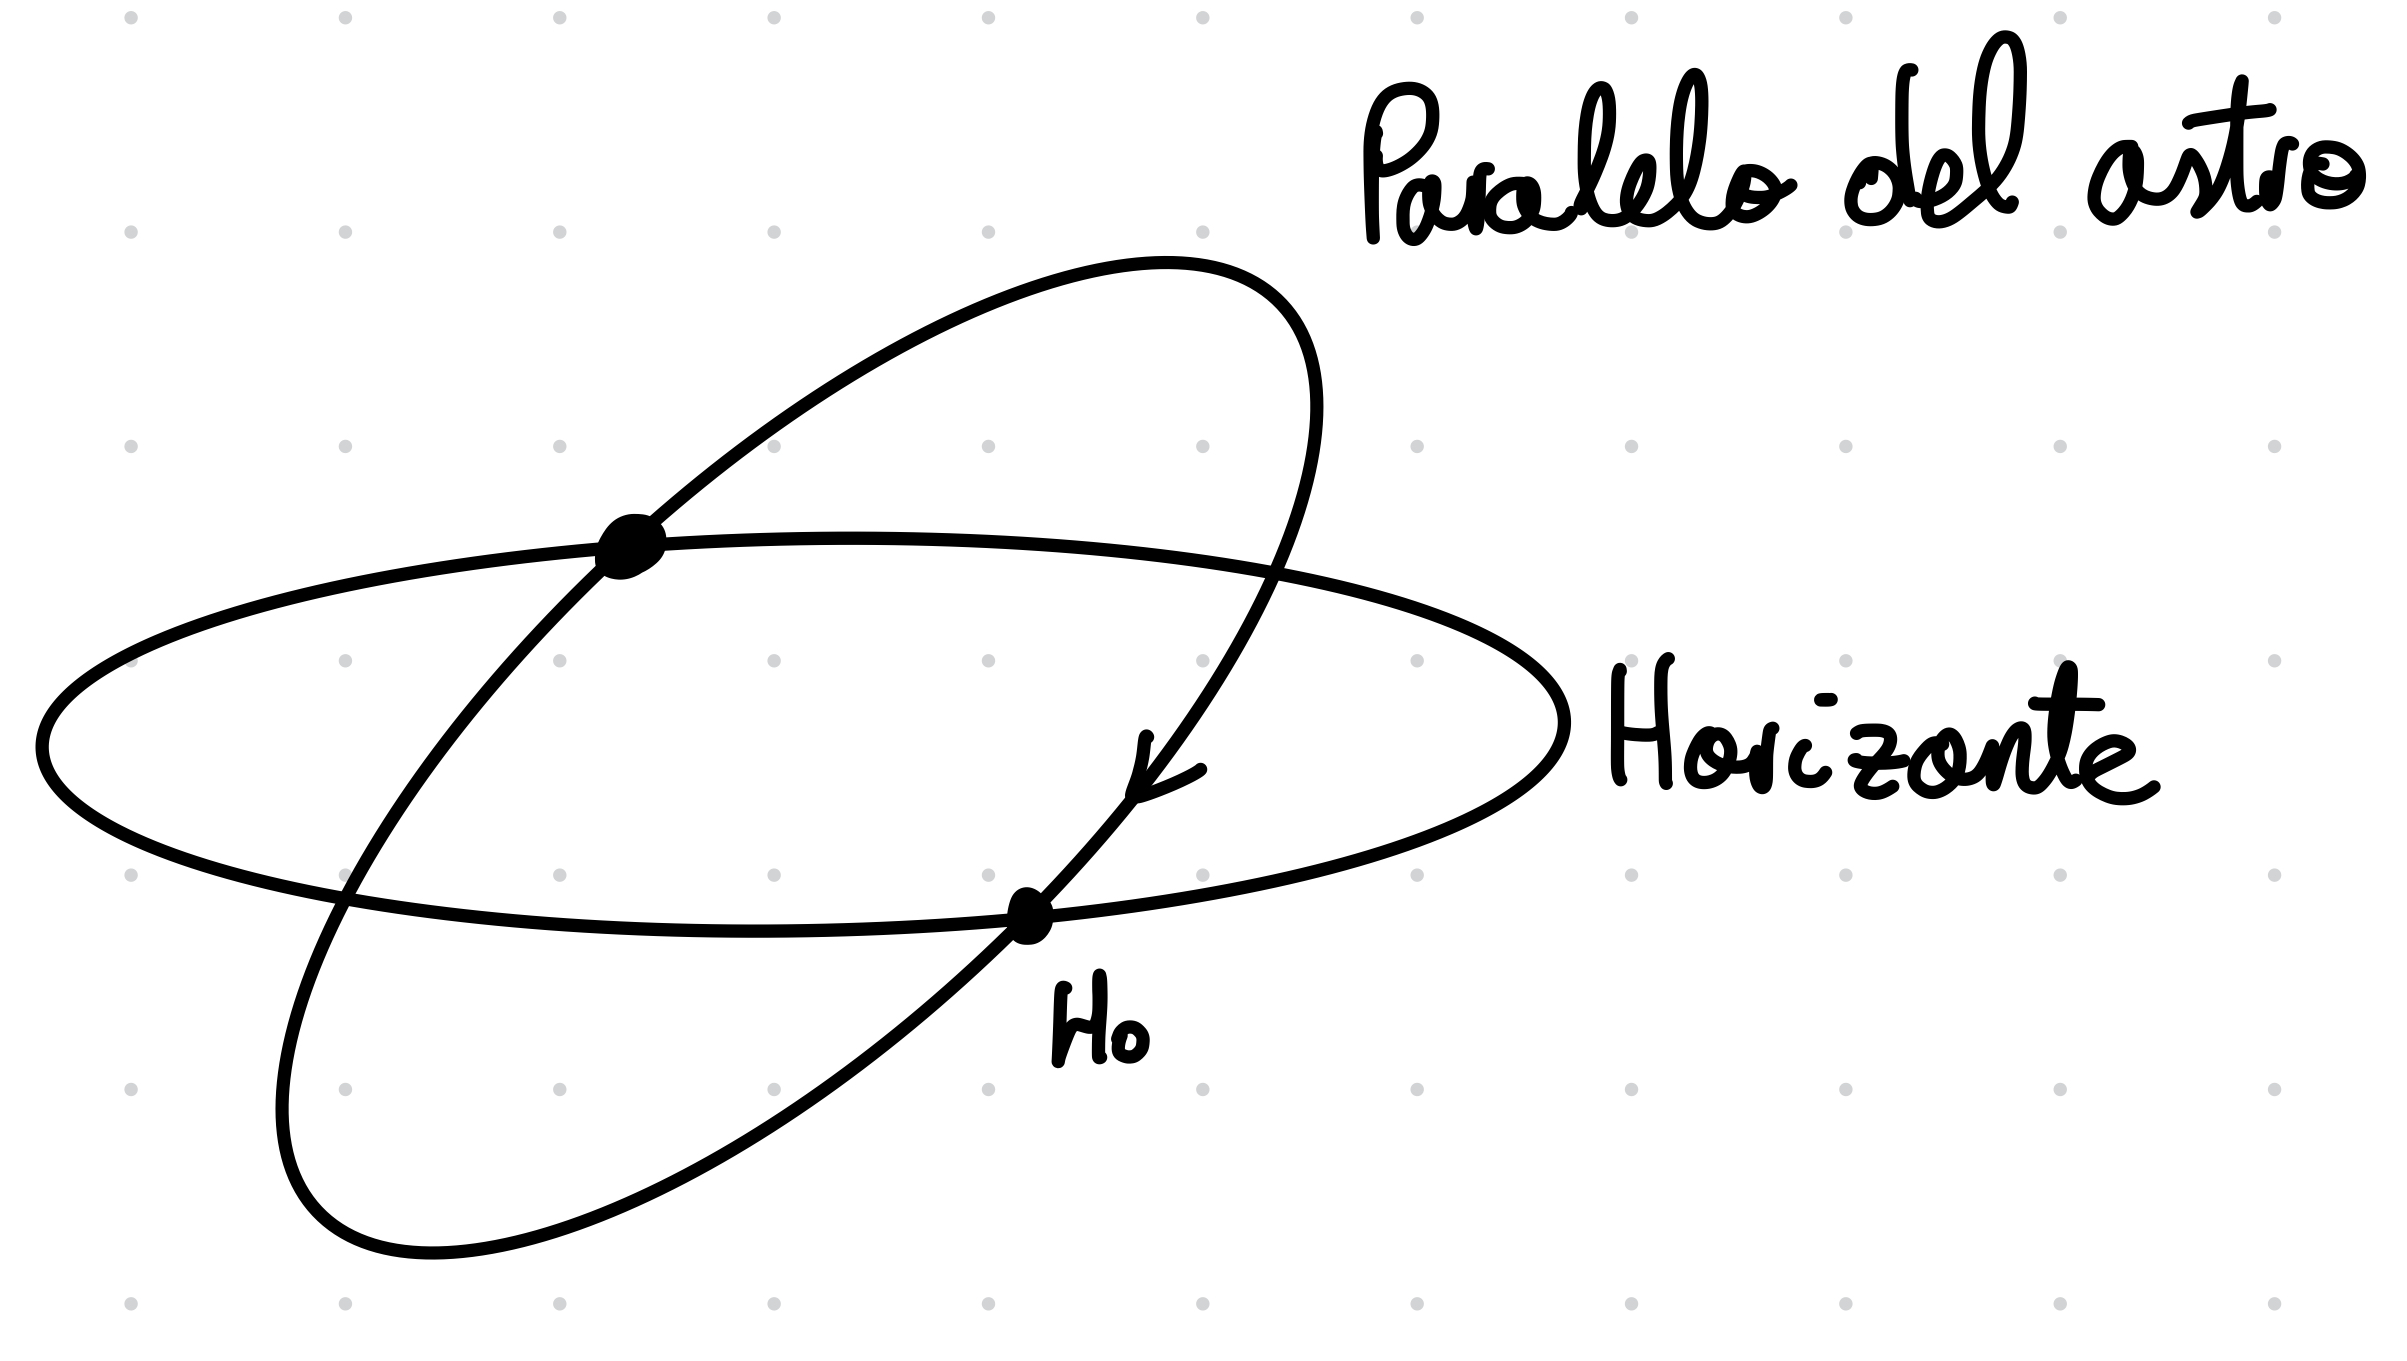
\includegraphics[width=1.0\textwidth]{Cuerpo/Imagenes/01_Ejercicio_2.jpg}
	 \end{minipage}
	
	
